\subsubsection{Uso de la aplicacion por personas sin español como idioma nativo}

{\textbf {Resumen:}}
Un usuario extranjero llega a un museo local es su ruta de turismo, al ver un cartel de la App en el museo la descarga, luego en su alojamiento decide probar la aplicación, al abrirla este se encuentra con una serie de imágenes que le muestran cómo ocupar la aplicación, estas imágenes están acompañadas de un texto en español pero el logra sin ningún problema a ocupar la aplicación.

{\textbf {Actores:}}
Usuario de nacionalidad extranjera (no chileno), Museo/Publicidad.

{\textbf {Propósito:}}
Lograr que una persona que no maneja el lenguaje nacional logre interactuar con la aplicación sin problemas, adems de demostrar su uso de manera internacional.

{\textbf {Referencias cruzadas:}}
R 1.1, R 1.2, R1.3, R3.4, R3.5

\paragraph{Caso de Uso Esencial}

\begin{longtable}{|p{5cm}|p{8cm}|}
\hline 
Acción actores & Respuesta del sistema \\ 
\hline 
XXXX & XXXX \\ 
\hline 
\end{longtable}

\paragraph{Diagrama de Caso de Uso}

\begin{figure}[H]
\centerline{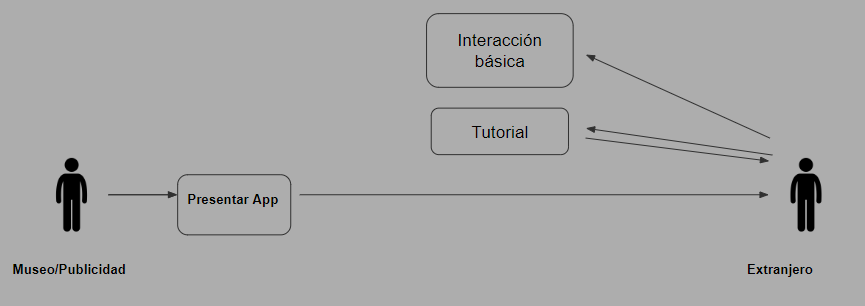
\includegraphics[width=15cm]{imgs/CasoUso_2.PNG}}
\caption{Caso-1}
\label{fig}
\end{figure}

\subsubsection{Modelo Conceptual}

\begin{figure}[H]
\centerline{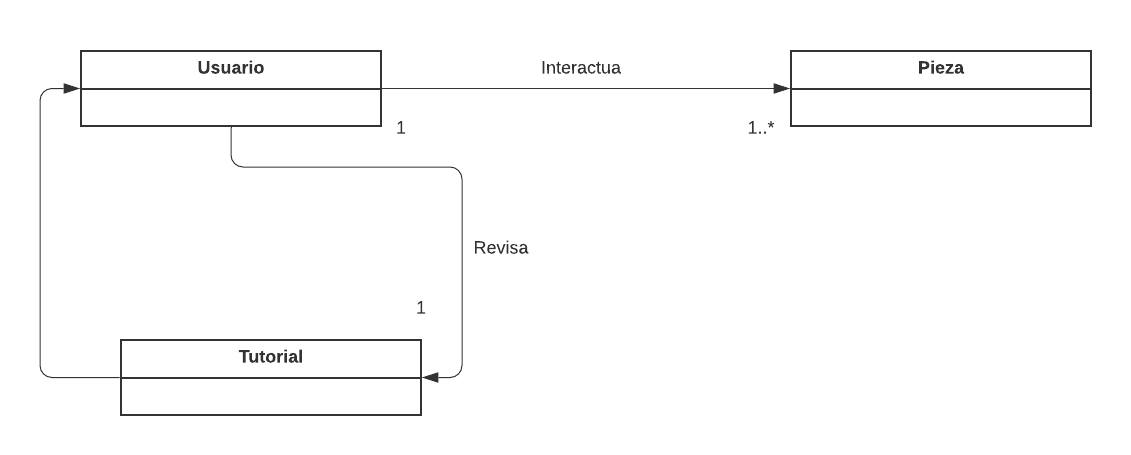
\includegraphics[width=15cm]{imgs/ModeloConceptualCaso_2_3.png}}
\caption{Caso-1}
\label{fig}
\end{figure}

\paragraph{Diagrama de Secuencia o Colaboración}

\begin{figure}[H]
\centerline{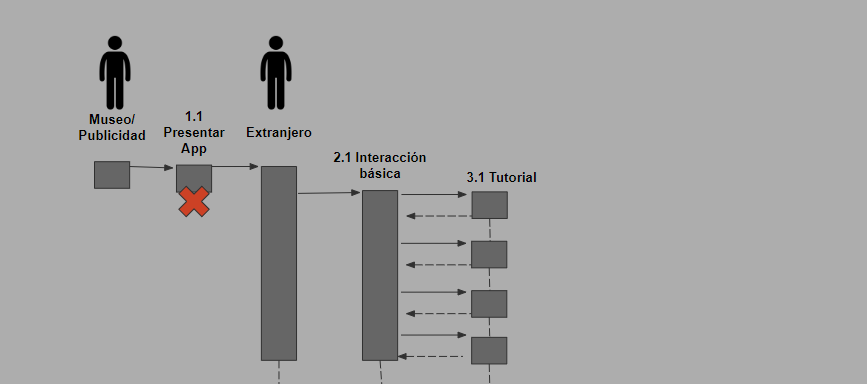
\includegraphics[width=15cm]{imgs/CasoUso_2_2.PNG}}
\caption{Caso-1}
\label{fig}
\end{figure}

\paragraph{Priorización}
{\textbf {Tipo:}}
Relevante.